\section{Gitlab CI/CD}

\begin{frame}
\frametitle{Pipeline}
\begin{figure}
    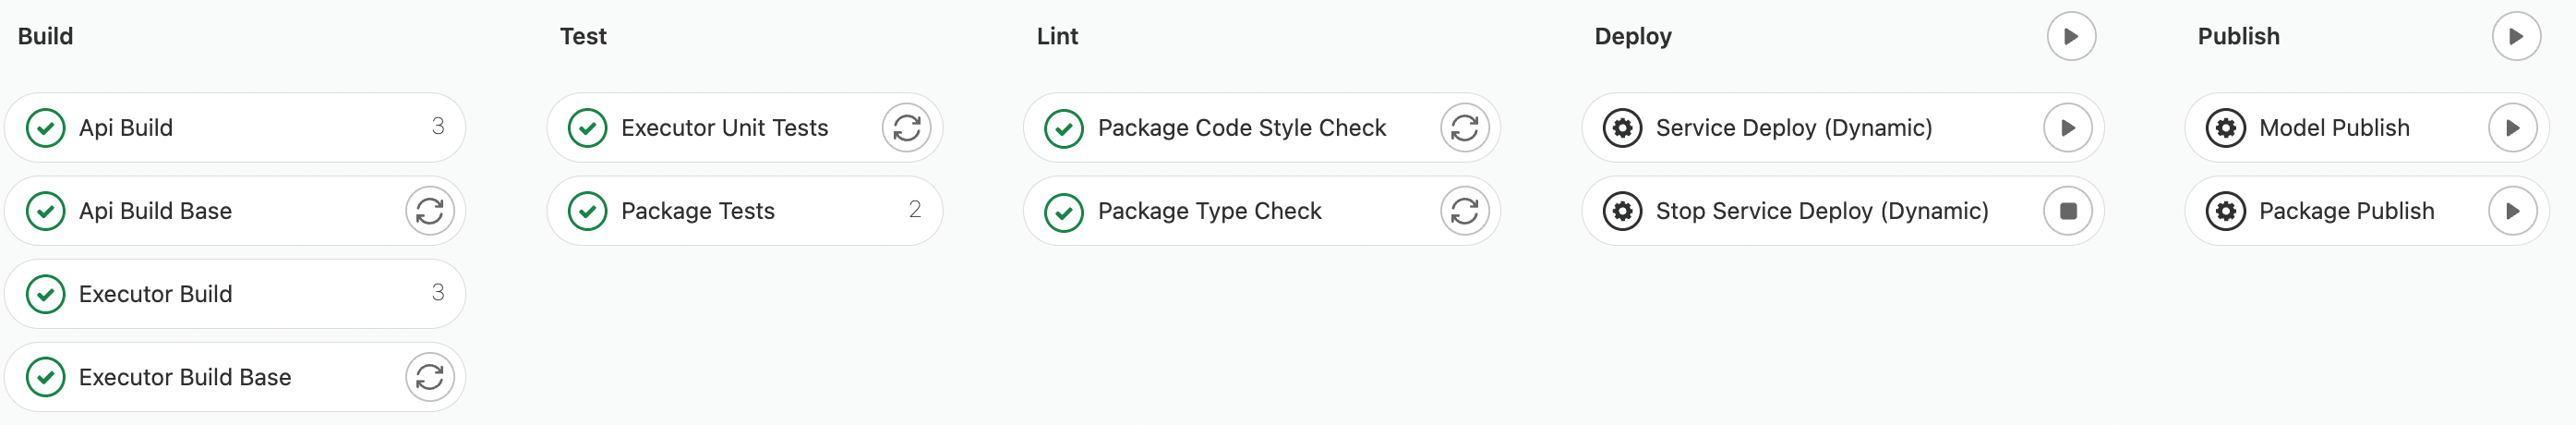
\includegraphics[scale=.3]{pictures/implementation/stages}
    \caption{Pipeline Gitlab CI/CD}
\end{figure}
\end{frame}

\begin{frame}
\frametitle{Зависимости}
\begin{figure}
    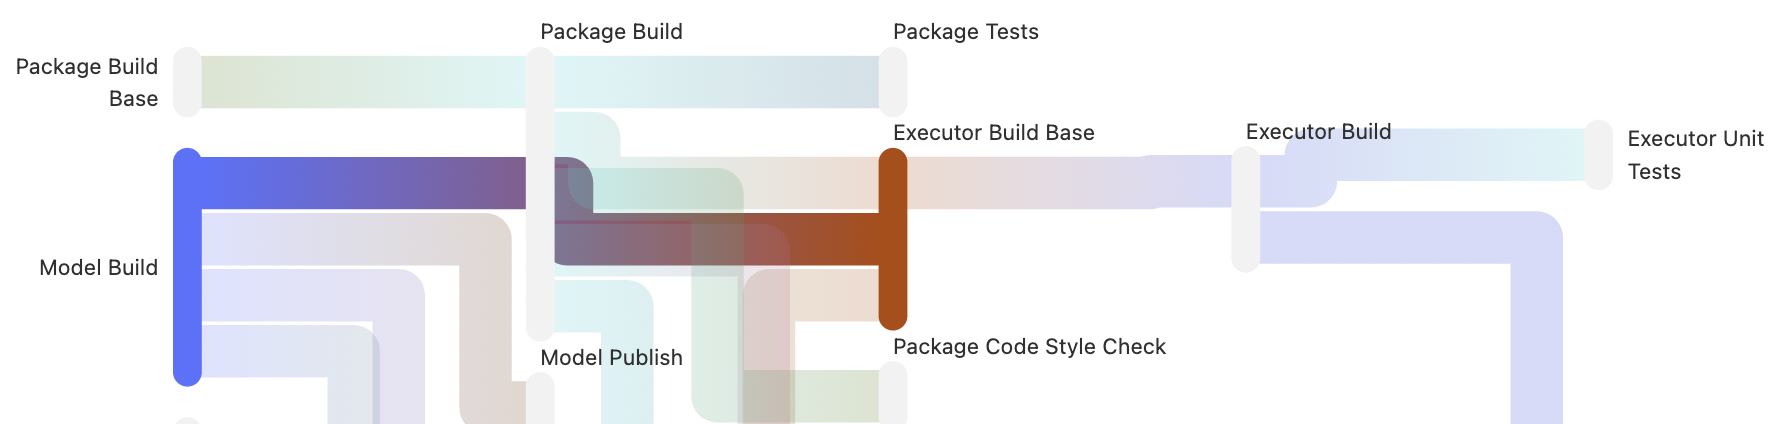
\includegraphics[scale=.45]{pictures/implementation/dependencies}
    \caption{Отображение зависимостей}
\end{figure}
\end{frame}


\begin{frame}
\frametitle{Тесты}
\begin{figure}
    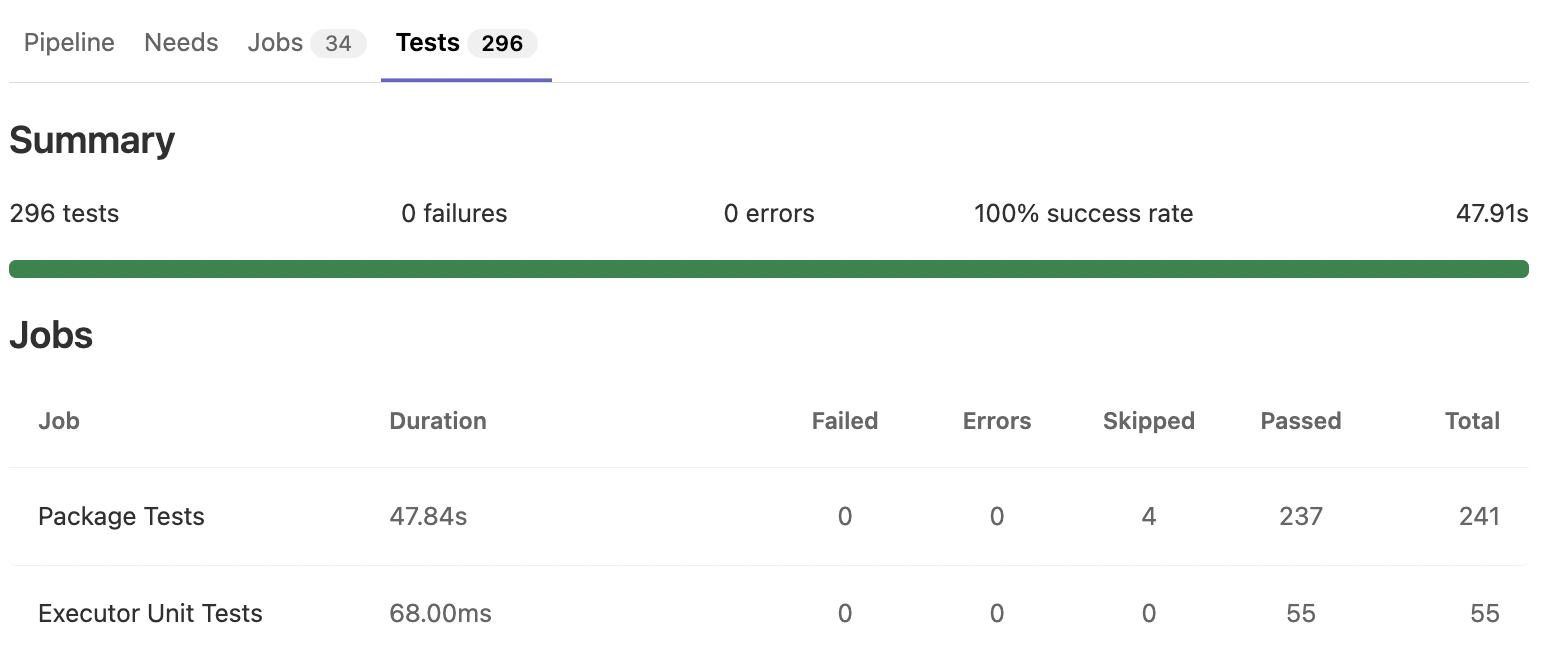
\includegraphics[scale=.4]{pictures/implementation/tests}
    \caption{Отображение тестов}
\end{figure}
\end{frame}


\begin{frame}
\frametitle{Окружения}
\begin{figure}
    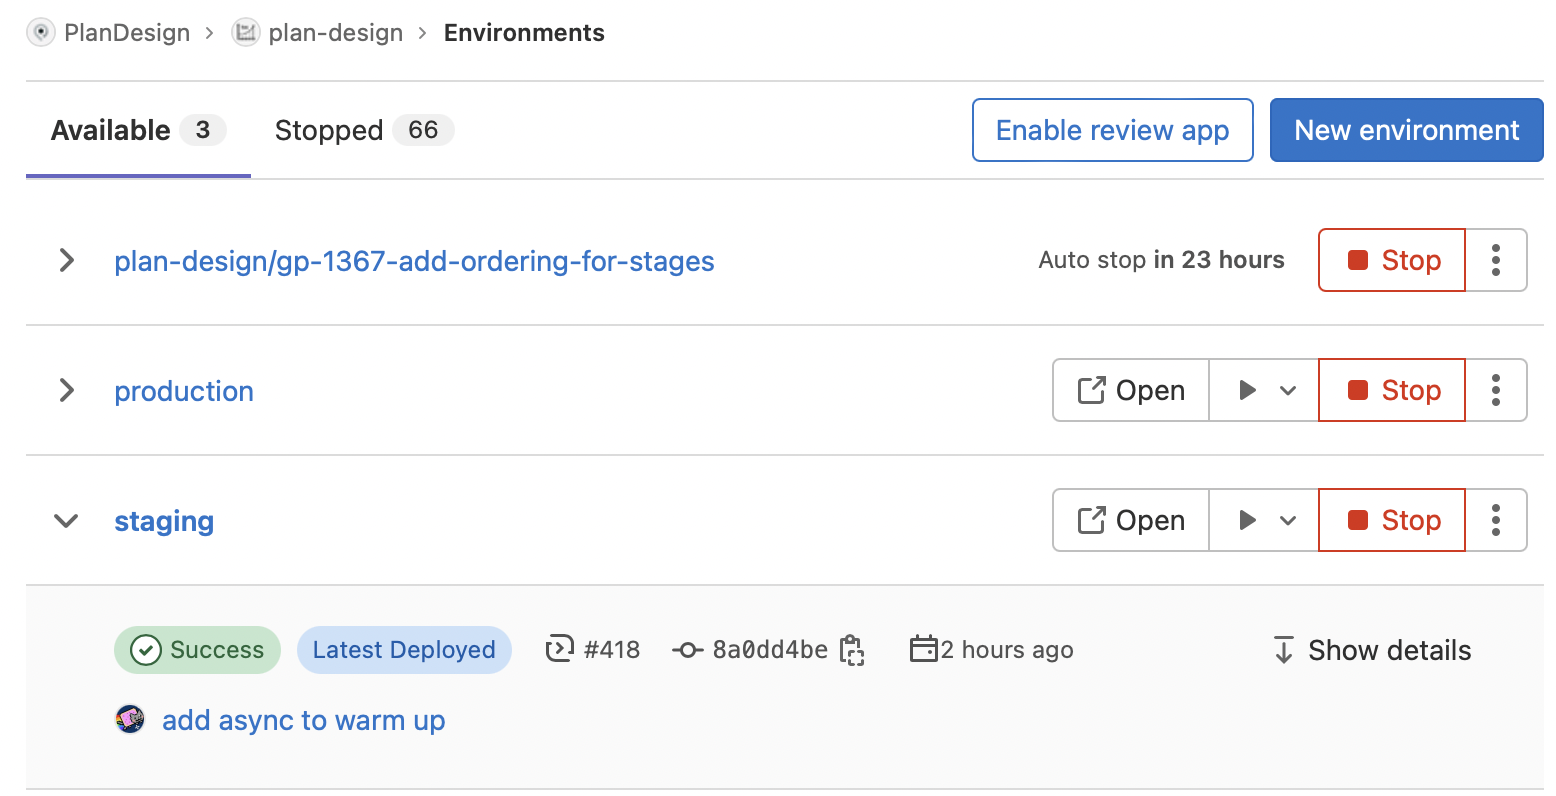
\includegraphics[scale=.45]{pictures/implementation/environment}
    \caption{Пример интерфейса Environments}
\end{figure}
\end{frame}



